

 En este capítulo se comentará el proceso seguido para la realización de este proyecto detallando la planificación, diseño y el desarrollo del mismo estructurado en etapas.
 
\section{Planificación}

Una vez hecho el análisis, conocidos los objetivos que se quieren alcanzar en este proyecto y las herramientas que se utilizarán  empezaremos con la planificación del mismo.

Un punto muy  importante a tener en cuenta a la hora de realizar una planificación sería conocer los recursos y el tiempo del que disponemos.




Éste punto tan crucial se acentúa ya que este proyecto será hecho por una única persona lo que producirá sobrecargas en la planificación. Esto normalmente no es así ya que los proyectos se realizan por grupos de trabajos y muchas tareas pueden realizarse en paralelo disminuyendo apreciablemente la duración del proyecto.

Para realizar la planificación del proyecto hemos dividido el proyecto en tareas con unos objetivos bien marcados. A su vez al seguir la metodología Scrum dividimos el proyecto en etapas(Sprint) de tiempo  donde incluimos las tareas a realizar.
En todas estas etapas incluimos los siguientes pasos:
 
 


\begin{itemize}
\item Creación del  backlog, lista de tarea que vamos a realizar en cada Sprint.




\item  División de las tareas en tareas más sencillas y más fáciles de manejar.



\item Diseño de cada una de las tareas del punto anterior.
\item  Implementacion de las tareas.
\item Pruebas.
\end{itemize}



\section{Estimación de tiempos y costes}
 A continuación en la tabla siguiente se ha realizado una estimación de tiempos y de costes de este proyecto.
 Cuando se realiza una estimación de costes tenemos que tener en cuenta los gastos en material, licencias y los gastos propios. En este caso los gastos de materias y de licencias en cero ya que el material usado era todo el alumno y las licencias eran todas gratuitas.
 En la siguiente tabla se detalla el esfuerzo horas-hombre de cada uno de los roles dentro del proyecto. Para calcular los costes de los recursos humanos, se han usados los salarios medios de cada uno de los roles en Galicia y que no están incluidos beneficios exclusivamente los costes. 
 
 
 
\begin{figure}[H]
		\centering
		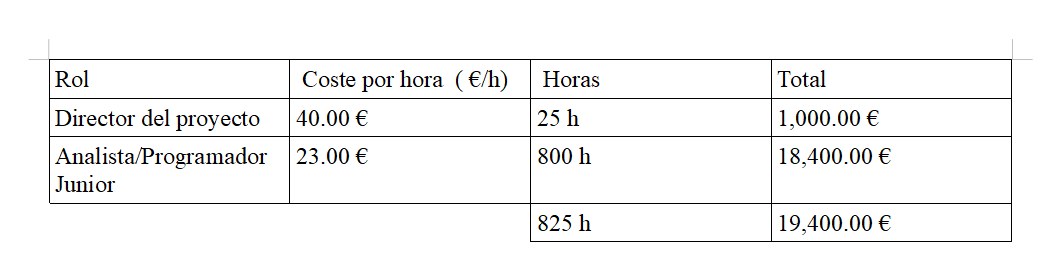
\includegraphics[width=0.75\textwidth] {coste.png}
		\caption{Costes asociados a este proyecto }
	\end{figure}






\begin{itemize}
\item En el rol de director de proyecto estarían los que 
supervisan y evalúan el proyecto. En este caso Javier y Óscar realizarán este rol.

\item Analista/programador, en este rol estaría la persona encargada de las tareas de análisis, diseño, desarrollo y de la creación de las pruebas para este proyecto. Al estar realizado por mi yo haría de este rol.




 Tendo en conta unha
xornada laboral de 6 horas e que a duracion de cada Sprint e de 15 das podemos estimar
o custo total do proxecto en:
\end{itemize}
\section{Seguimiento}
Como se comentou na seccion de metodoloxa o proxecto realzase en Sprints. Denimos
un total de oito Sprints, cunha duracion xa de 15 das, no que se atopan denidos
as tarefas a realizar. A continuacion detallanse os Sprints que se realizaron o longo do
proxecto.